\documentclass[12pt]{article}

\usepackage{graphicx}
\usepackage{paralist}
\usepackage{amsfonts}
\usepackage{amsmath}
\usepackage{hhline}
\usepackage{booktabs}
\usepackage{multirow}
\usepackage{multicol}
\usepackage{url}
\usepackage{hyperref}

\oddsidemargin -10mm
\evensidemargin -10mm
\textwidth 160mm
\textheight 200mm
\renewcommand\baselinestretch{1.0}

\pagestyle {plain}
\pagenumbering{arabic}

\newcounter{stepnum}

\usepackage{color}

\newif\ifcomments\commentstrue

\ifcomments
\newcommand{\authornote}[3]{\textcolor{#1}{[#3 ---#2]}}
\newcommand{\todo}[1]{\textcolor{red}{[TODO: #1]}}
\else
\newcommand{\authornote}[3]{}
\newcommand{\todo}[1]{}
\fi

\newcommand{\wss}[1]{\authornote{blue}{SS}{#1}}

\title{AutoChecker, Specification}
\author{Ricky Fan, HaoWei Chen}

\begin {document}

\maketitle
\noindent This Module Interface Specification (MIS) document contains modules, types and
methods used to support the AutoChecker. The AutoChecker start by prompting the user to select a 
checker mode (single file vs multi-files). If the single file mode is selected, the user will be 
prompted to enter two file directories, their corresponding sheets and column headers. Then the 
checker will output a list of rows with different values. If the multi-files mode is selected, 
then user will be prompted to enter multiple (default $5$) file directories, their corresponding 
sheets and column headers. Later, the user will be prompted to enter another file directory 
and its corresponding sheet and column header. Then, the checker will use the data from these 
files to output a list of rows with different values
\texttt{make demo} in terminal.

\newpage

\section{Overview of the design}

This design applies Module View Specification (MVC) design pattern and 
Singleton design pattern. The MVC components are \textit{Checker} (model module), 
\textit{View} (view module), and \textit{Controller} (controller module). Singleton pattern is 
specified and implemented for \textit{View} and \textit{Controller} 

\bigskip

\noindent An UML diagram is provided below for visualizing the structure of this software architecture

\begin{center}
  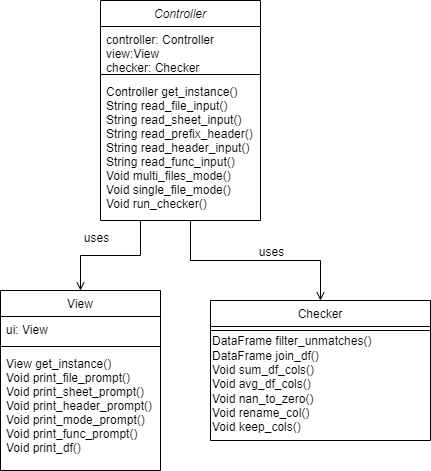
\includegraphics[width=0.6\textwidth]{UML_AutoChecker.png}
\end{center}

\medskip

\noindent The MVC design pattern are specified and implemented in the following way: 
the abstract object \textit{Checker} compare, aggregate and transform the data gather 
from external (excel) files. A view module \textit{View} displays prompt messages and 
rows with different values. The controller \textit{Controller} is responsibe for handling 
input actions and the control flow of the automation

\medskip

\noindent For \textit{View} and \textit{Controller}, use the get\_instance() method to obtain the abstract object.

\newpage

\section* {Checker Module (Abstract Object)}

\subsection*{Module}

Checker

\subsection* {Uses}

pandas

\subsection* {Syntax}

\subsubsection* {Exported Constants}

None

\subsubsection* {Exported Types}

Checker = ?

\subsubsection* {Exported Access Programs}

\begin{tabular}{| l | l | l | p{5cm} |}
\hline
\textbf{Routine name} & \textbf{In} & \textbf{Out} & \textbf{Exceptions}\\
\hline
filter\_unmatches & DataFrame, String, String & DataFrame & \\
\hline
join\_df & DataFrame, DataFrame, String & DataFrame & \\
\hline
sum\_df\_cols & DataFrame, $\mathbb{N}$, $\mathbb{N}$, String & & \\
\hline
avg\_df\_cols & DataFrame, $\mathbb{N}$, $\mathbb{N}$, String & & \\
\hline
% \hline
% get\_unmatches & $\text{seq of } \mathbb{N}$, $\text{seq of } \mathbb{N}$ & $\text{seq of (seq of } \mathbb{N} \text{)}$ & \\
% \hline
% agg\_cols & $\text{seq of (seq of } \mathbb{N} \text{)}$, $\text{seq of } \mathbb{N} \rightarrow \mathbb{N}$ & $\text{seq of } \mathbb{N}$ & \\
% \hline
% trans\_mat & $\text{seq of (seq of } \mathbb{N} \text{)}$ & & \\
% \hline

\end{tabular}

\subsection* {Semantics}

\subsubsection* {State Variables}

None

\subsubsection* {State Invariant}

None

\subsubsection* {Assumptions}

None

\subsubsection* {Access Routine Semantics}

\noindent filter\_unmatches(df, col1, col2):
\begin{itemize}
    \item output: filter out every row in the DataFrame that has different values in the two specified columns
    \item exception: none
\end{itemize}

\noindent join\_df(df1, df2, key):
\begin{itemize}
    \item output: inner join two DataFrames on the specified key
    \item exception: none
\end{itemize}

\noindent sum\_df\_cols(df, start\_idx, end\_idx, col\_name):
\begin{itemize}
    \item transition: add an additional column with the input name to the DataFrame that stores the sum of 
    every row from the specified starting index to the ending index
    \item exception: none
\end{itemize}

\noindent avg\_df\_cols(df, start\_idx, end\_idx, col\_name):
\begin{itemize}
    \item transition: add an additional column with the input name to the DataFrame that stores the average of 
    every row from the specified starting index to the ending index
    \item exception: none
\end{itemize}

% \noindent get\_unmatches(col1, col2):
% \begin{itemize}
%     \item output: out $:= [ i: \mathbb{N} | i \in \{0 .. |\text{col}1|-1\} : \text{col}1[i] \neq \text{col}2[i] \Rightarrow [ i,  \text{col}1[i], \text{col}2[i]] ]$
%     \item exception: none
% \end{itemize}

% \noindent agg\_cols(cols, func):
% \begin{itemize}
%     \item output: out $:= [ i: \mathbb{N} | i \in \{0 .. |\text{cols}|-1\} : \text{func(cols}[i]\text{)} ]$
%     \item exception: none
% \end{itemize}

% \noindent trans\_mat(matrix):
% \begin{itemize}
%     \item transition: $\forall i : \mathbb{N} \; | \; i < |\text{matrix}| $ $\wedge$ 
%     ($\forall j : \mathbb{N} \; | \; i \le j < |\text{matrix}[i]|$ $\wedge$ tr\_swap($i$, $j$))
%     \item exception: none
% \end{itemize}

% \subsubsection*{Local Function:}

% % \noindent transMat: seq of (seq of $\mathbb{N}$)\\
% % transMat(matrix): $\forall$ $i : \mathbb{N}$ $|$ $i < |\text{matrix}| $ $\wedge$ 
% % ($\forall$ $j : \mathbb{N}$ $|$ $i \le j < |\text{matrix}[i]|$ $\wedge$ $\text{trSwap}(i, j)$)\\

% \noindent tr\_swap: seq of (seq of $\mathbb{N}$) $\times \mathbb{N} \times \mathbb{N} \rightarrow$ void\\
% \noindent tr\_swap(matrix, row, col): 
% \begin{itemize}[\null]
%   \item tmp $:=$ matrix[row][col]
%   \item matrix[row][col] $:=$ matrix[col][row]
%   \item matrix[col][row] $:=$ tmp
% \end{itemize}

\newpage

\section* {View Module}

\subsection*{Module}

View

\subsection* {Uses}

None

\subsection* {Syntax}

\subsubsection* {Exported Constants}

None

\subsubsection* {Exported Types}

None

\subsubsection* {Exported Access Programs}

\begin{tabular}{| l | l | l | p{5cm} |}
  \hline
  \textbf{Routine name} & \textbf{In} & \textbf{Out} & \textbf{Exceptions}\\
  \hline
  get\_instance &  & View & \\
  \hline
  print\_file\_prompt & &  & \\
  \hline
  print\_sheet\_prompt & & & \\
  \hline
  print\_header\_prompt & & & \\
  \hline
  print\_mode\_prompt & & & \\
  \hline
  print\_func\_prompt & & & \\
  \hline
  print\_df & DataFrame & & \\
  \hline

\end{tabular}

\subsection* {Semantics}

\subsection*{Environment Variables}

window: A portion of computer screen to display the messages (i.e. the terminal)

\subsubsection* {State Variables}

ui: View

\subsubsection* {State Invariant}

None

\subsubsection* {Assumptions}

\begin{itemize}
  \item The View constructor is called for each object instance before any 
  other access routine is called for that object.  
  \item The constructor can only be called once.
\end{itemize}


\subsubsection* {Access Routine Semantics}

\noindent get\_instance():
\begin{itemize}
\item transition: ui $:=$ (ui = null $\Rightarrow$ new View())
\item output: \textit{self}
\item exception: none
\end{itemize}

\noindent print\_file\_prompt():
\begin{itemize}
\item transition: window $:=$ Displays a prompt message asking the user to enter a file directory
\end{itemize}

\noindent print\_sheet\_prompt():
\begin{itemize}
\item transition: window $:=$ Displays a prompt message asking the user to enter a sheet name
\end{itemize}

\noindent print\_header\_prompt():
\begin{itemize}
\item transition: window $:=$ Displays a prompt message asking the user to enter a header name
\end{itemize}

\noindent print\_mode\_prompt():
\begin{itemize}
\item transition: window $:=$ Displays a prompt message asking the user to select a checker mode
\end{itemize}

\noindent print\_func\_prompt():
\begin{itemize}
\item transition: window $:=$ Displays a prompt message asking the user to select a function
\end{itemize}

\noindent print\_df(df):
\begin{itemize}
\item transition: window $:=$ Displays the DataFrame
\end{itemize}

\subsubsection*{Local Function:}

\_\_init\_\_: void $\rightarrow$ View \\
\_\_init\_\_() $\equiv$ new View()

\newpage

\section* {Controller Module}

\subsection* {Controller Module}

\subsection* {Uses}

Checker, View, pandas

\subsection* {Syntax}

\subsubsection* {Exported Types}

None

\subsubsection* {Exported Constants}

None

\subsubsection* {Exported Access Programs}

\begin{tabular}{| l | l | l | p{4.7cm} |}
\hline
\textbf{Routine name} & \textbf{In} & \textbf{Out} & \textbf{Exceptions}\\
\hline
get\_instance & View & Controller & \\
\hline
read\_file\_input & & String & \\
\hline
read\_sheet\_input & & String & \\
\hline
read\_header\_input & & String & \\
% \hline
% load\_xlsx & Strint, String & DataFrame & FileNotFoundException \\ 
%            &                &           & SheetNotFoundException \\ 
%            &                &           & FileNotSupportException \\
\hline
read\_func\_input & & String & \\
\hline
multi\_file\_mode & Map of String and String & &\\
                  & Pair of String and Map &  & \\
\hline
single\_file\_mode & Pair of String and Map & &\\
                   & Pair of String and Map & & \\
\hline
run\_checker & & & \\
\hline
\end{tabular}

\subsection* {Semantics}

\subsection*{Environment Variables}

None

\subsubsection* {State Variables}

view: View \\
controller: Controller

\subsubsection* {State Invariant}

None

\subsubsection* {Assumptions}

\begin{itemize}
  \item The Controller constructor is called for each object instance before any
  other access routine is called for that object.  
  \item The constructor can only be called once.
  \item Assume that the view instances are already initialized before calling 
  Controller constructor
\end{itemize}

\subsubsection* {Access Routine Semantics}

get\_instance($v$):
\begin{itemize}
  \item transition: controller $:=$ (controller = null $\Rightarrow$ new Controller ($v$))
  \item output: \textit{self}
  \item exception: None
\end{itemize}

\noindent read\_file\_input():
\begin{itemize}
  \item output: $input$ : String, file directory entered by the User
  \item exception: none
\end{itemize}

\noindent read\_sheet\_input():
\begin{itemize}
  \item output: $input$ : String, sheet name entered by the User
  \item exception: none
\end{itemize}

\noindent read\_header\_input():
\begin{itemize}
  \item output: $input$ : String, column header entered by the User
  \item exception: none
\end{itemize}

\noindent read\_mode\_input():
\begin{itemize}
  \item output: $input$ : String, mode selected by the User
  \item exception: none
\end{itemize}

\noindent read\_func\_input():
\begin{itemize}
  \item output: $input$ : String, function selected by the User
  \item exception: none
\end{itemize}

\noindent single\_file\_mode(file1, file2):
\begin{itemize}
  \item transition: operational method 
  \begin{itemize}[\null]
    \item df1 $:=$ get\_df\_col(file1[$0$], file1[$1$])
    \item df2 $:=$ get\_df\_col(file2[$0$], file2[$1$])
    \item dfj $:=$ Checker.join\_df(df1, df2, 'prefix') 
    \item df\_umatches $:=$ Checker.filter\_unmatches(dfj, file1[$1$]['header'], file2[$1$]['header'])
    \item view.print\_df(df\_unmatches)
  \end{itemize}
  \item output: none
\end{itemize}

\noindent multi\_files\_mode(f\_map, file2):
\begin{itemize}
  \item transition: operational method 
  \begin{itemize}[\null]
    \item f\_arr $:=$ [$f$:String $|$ $f \in$ f\_map.keys() $:$ get\_df\_col($f$, f\_map[$f$]) ]
    \item df\_mult $:=$ f\_arr[$0$]
    \item df\_mult $:=$ (Check.join\_df(df\_join, f\_arr[i]) DataFrame, 
    $i:\mathbb{N}$ $|$ $i \in \{1..|f\_arr|-1\}$ $:$ f\_arr[i])
    \item view.print\_func\_prompt()
    \item input\_func $:=$ read\_func\_input()
    \item input\_func $=$ 'sum' $\Rightarrow$ sum\_df\_cols(df\_mult, $1$, $|f\_arr|-1$, input\_func) $|$  
    input\_func $=$ 'avg' $\Rightarrow$ av\_df\_cols(df\_mult, $1$, $|f\_arr|-1$, input\_func)
    \item df2 $:=$ get\_df\_col(file2[$0$], file2[$1$])
    \item df\_join $:=$ Checker.join\_df(df\_mult, df2,' prefix') 
    \item df\_unmatches $:=$ Checker.filter\_unmatches(df\_join, input\_func, file2[$1$]['header'])
    \item view.print\_df(df\_unmatches)
  \end{itemize}
  \item output: none
\end{itemize}

\noindent run\_checker():
\begin{itemize}
  \item transition: operational method for running the game. \\
  Start by prompting the user to select the checker mode (single file vs multi files)
  \begin{itemize}
    \item If single file mode is selected:
      \begin{itemize}[\null]
        \item $f1$ $:=$ () 
        \item $f2$ $:=$ ()
        \item populate\_pair($f1$)
        \item populate\_pair($f2$)
        \item single\_file\_mode($f1$, $f2$)
      \end{itemize}
    \item If multi files mode is selected:
      \begin{itemize}[\null]
        \item $f\_map$ $:=$ \{\}
        \item $f1$ $:=$ () 
        \item populate\_pair($f1$)
        \item inputs $:=$ get\_inputs()
        \item f\_map[inputs[$0$]] $=$ \{'sheet':inputs[$1$], 'header':inputs[$2$]\}
        \item populate f\_map by repeating step $3$ - $4$ five times
        \item multi\_files\_mode($f\_map$, $f1$)
      \end{itemize}
  \end{itemize}

  \item output: None
\end{itemize}

\subsubsection*{Local Function:}

\_\_init\_\_: View $\rightarrow$ Controller \\
\_\_init\_\_($view$) $\equiv$ new Controller($view$) \\

% \noindent cal\_sum: seq of $\mathbb{N} \rightarrow \mathbb{N}$\\
% cal\_sum(seq) $\equiv (+s:\mathbb{N} \; | \; s \in \text{seq} : s)$ \\

% \noindent cal\_avg: seq of $\mathbb{N} \rightarrow \mathbb{N}$\\
% cal\_avg(seq) $\equiv \text{cal\_sum}(seq) / |\text{seq}|$\\

\noindent get\_df\_col: String $\times$ Map of String and String $\rightarrow$ DataFrame\\
get\_df\_col(file\_dir, info\_map):
\begin{itemize}[\null]
  \item df $:=$ load\_xlsx(file\_dir, info\_map['sheet'])
  \item out $:=$ df[[prefix, info\_map['header']]]
\end{itemize}

\noindent get\_inputs: seq of String\\
get\_inputs(p): 
\begin{itemize}[\null]
  \item view.print\_file\_prompt()
  \item file\_dir $:=$ read\_file\_input()
  \item view.print\_sheet\_input()
  \item sheet $:=$ read\_sheet\_input()
  \item view.print\_header\_input()
  \item header $:=$ read\_header\_input()
  \item out $:=$ [file\_dir, sheet, header]
\end{itemize}

\noindent populate\_pair: Pair $\rightarrow$ void\\
populate\_pair(p): 
\begin{itemize}[\null]
  \item inputs $:=$ get\_inputs()
  \item $p[0] :=$ inputs[$0$]
  \item $p[1] :=$ \{'sheet':inputs[$1$], 'header':inputs[$2$]\}
\end{itemize}

\noindent load\_xlsx: String $\times$ String $\rightarrow$ DataFrame\\
load\_xlsx(file\_dir, sheet\_name) $\equiv$ pandas.read\_excel(file\_dir, sheet\_name)

\end {document}